\section{Multiview Keypoint Reconstruction (Extra Credit)}
\label{sec:kps_recon}
You will use multi-view capture of moving vehicles and reconstruct the motion of a car. The first part of the problem will be using a single time instance capture from three views (\autoref{fig:q6} Top) and reconstruct vehicle keypoints and render from multiple views (\autoref{fig:q6} Bottom). Make use of\\\texttt{q6\_ec\_multiview\_reconstruction.py} file and \texttt{data/q6} folder contains the images.

\begin{figure}[t]
    \centering
    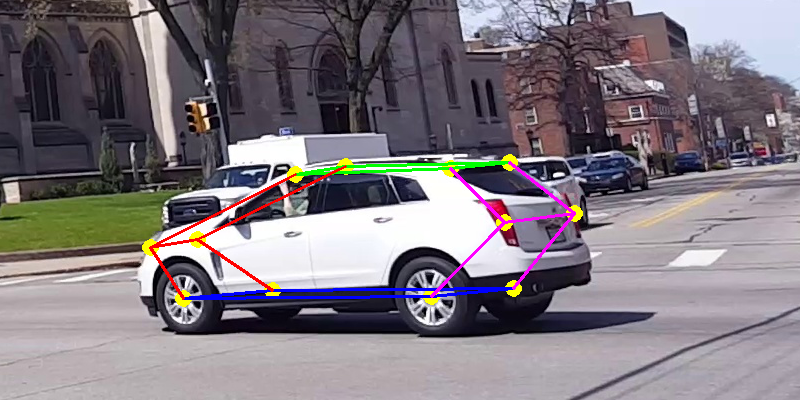
\includegraphics[width=0.32\textwidth]{images/q6/cam1_time4_det.png}
    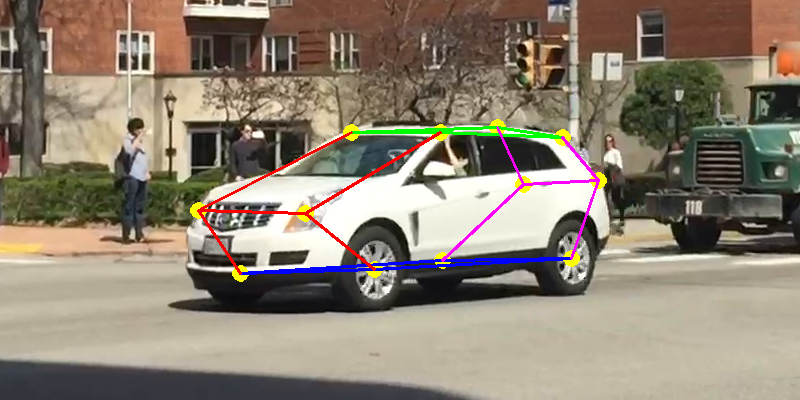
\includegraphics[width=0.32\textwidth]{images/q6/cam2_time4_det.png}
    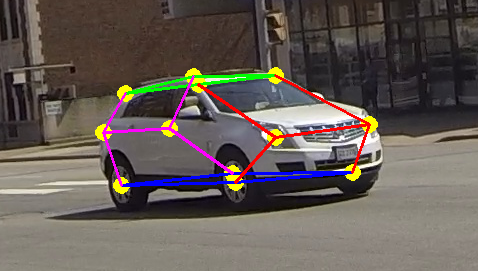
\includegraphics[width=0.32\textwidth]{images/q6/cam3_time4_det.png}\\
    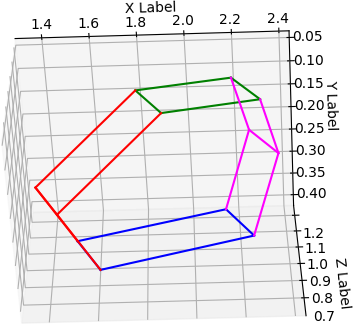
\includegraphics[width=0.32\textwidth]{images/q6/time4_recon_1.png}
    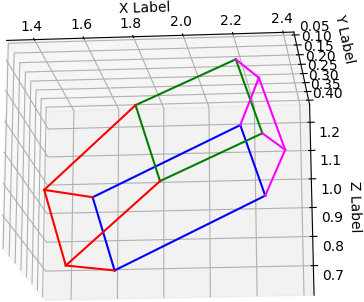
\includegraphics[width=0.32\textwidth]{images/q6/time4_recon_2.png}
    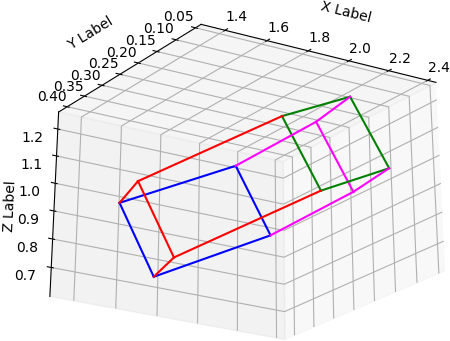
\includegraphics[width=0.32\textwidth]{images/q6/time4_recon_3.png}
    \caption{An example detections on the top and the reconstructions from multiple views}
    \label{fig:q6}
\end{figure}

\subparagraph*{Q6.1}\points{Extra Credit - 15}
Write a function to compute the 3D keypoint locations \texttt{P} given the 2D part detections \texttt{pts1}, \texttt{pts2} and \texttt{pts3} and the camera projection matrices \texttt{C1}, \texttt{C2}, \texttt{C3}. The camera matrices are given in the numpy files. 

\begin{center}
\texttt{[P, err] = MultiviewReconstruction(C1, pts1, C2, pts2, C3, pts3, Thres)}
\end{center}

The 2D part detections (\texttt{pts}) are computed using a neural network\footnote{\href{http://www.cs.cmu.edu/~ILIM/projects/IM/CarFusion/cvpr2018/index.html}{Code Used For Detection and Reconstruction}} and correspond to different locations on a car like the wheels, headlights etc. The third column in \texttt{pts} is the confidence of localization of the keypoints. Higher confidence value represents more accurate localization of the keypoint in 2D. To visualize the 2D detections run \texttt{visualize\_keypoints(image, pts, Thres)} helper function. \texttt{Thres} is defined as the confidence threshold of the 2D detected keypoints. The camera matrices (\texttt{C}) are computed by running an SFM from multiple views and are given in the numpy files with the 2D locations. By varying confidence threshold \texttt{Thres} (.i.e. considering only the points above the threshold), we get different reconstruction and accuracy. Try varying the thresholds and analyze its effects on the accuracy of the reconstruction. \deliver{Save the best reconstruction (the 3D locations of the parts) from these parameters into a \texttt{q6\_1.npz} file.} 

\textbf{\textit{Hint:}} You can modify the triangulation function to take three views as input. After you do the threshold lets say m points lie above the threshold and n points lie below the threshold. Now your task is to use these m good points to compute the reconstruction. For each 3D location use two view or three view triangulation for intialization based on visibility after thresholding. 

\deliver{
\textbf{In your write-up}: 
\begin{itemize}
    \item Describe the method you used to compute the 3D locations.
    \item Include an image of the Reconstructed 3D points with the points connected using the helper function \texttt{plot\_3d\_keypoint(P)} with the reprojection error.
    \item Include the code snippets \texttt{MultiviewReconstruction} in your write-up.
\end{itemize}
}

\begin{your_solution}[title=Q6.1,height=5.5cm,width=\linewidth]
\end{your_solution}

\subparagraph*{Q6.2}\points{Extra Credit - 15}
\begin{figure}[t]
    \centering
    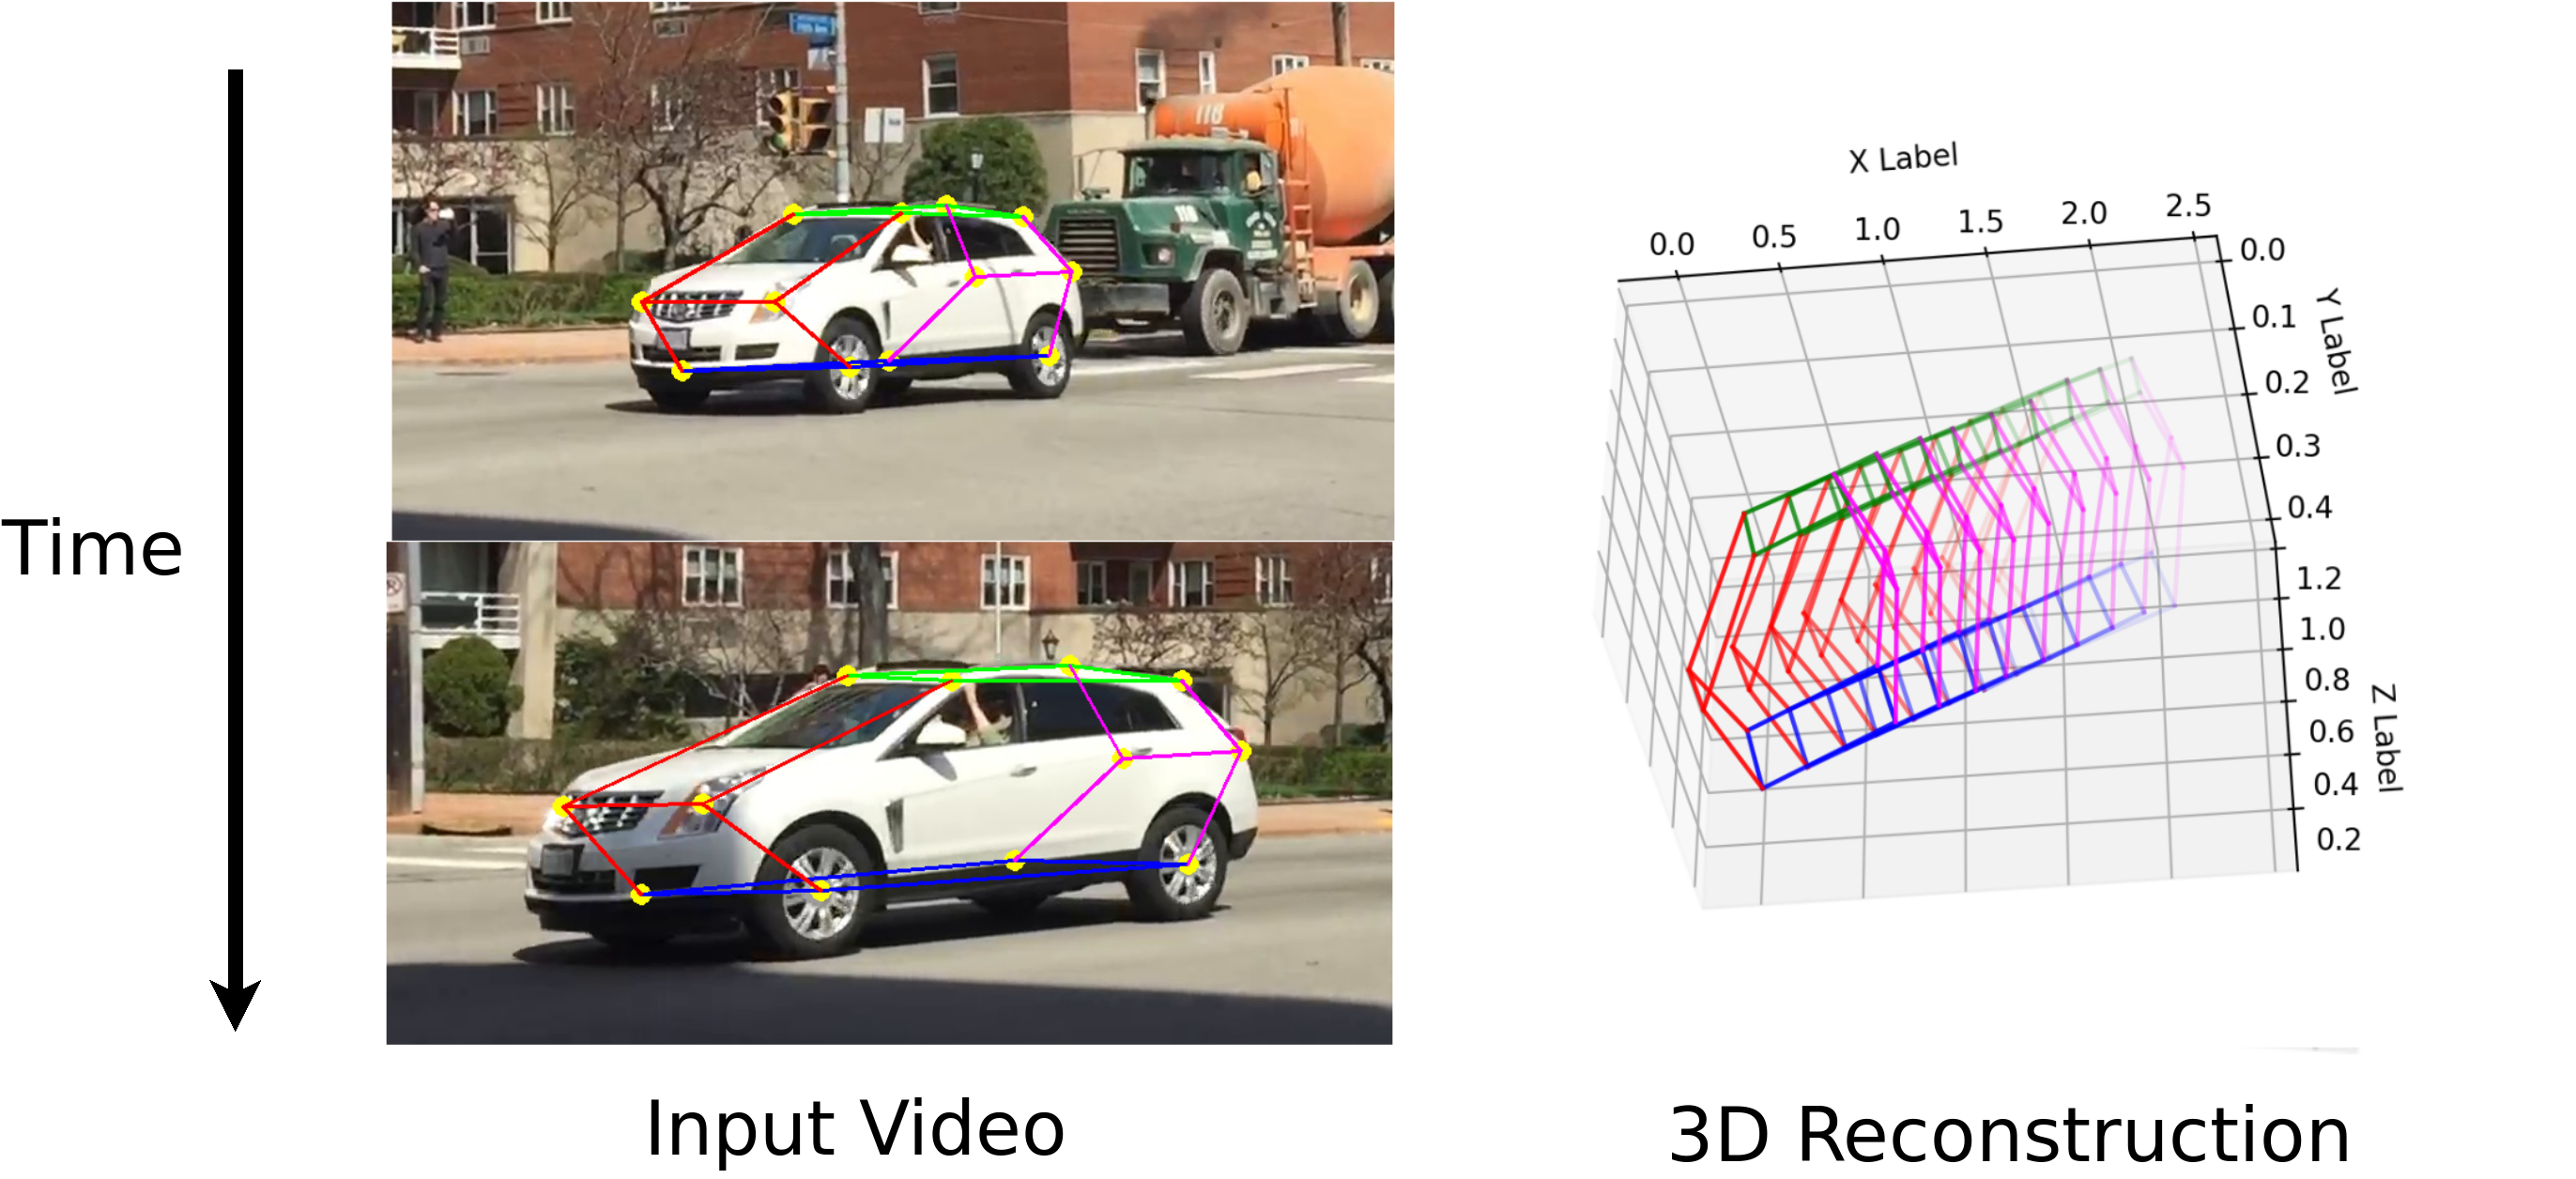
\includegraphics[width=\textwidth]{images/q6/temporal_new.png}
    \caption{Spatiotemporal reconstruction of the car (right) with the projections at two different time instances in a single view(left)}
    \label{fig:q6.2}
\end{figure}
From the previous question you have done a 3D reconstruction at a time instance. Now you are going to iteratively repeat the process over time and compute a spatio temporal reconstruction of the car. The images in the \texttt{data/q6} folder shows the motion of the car at an intersection captured from multiple views. The images are given as \texttt{(cam1\_time0.jpg, ..., cam1\_time9.jpg)} for camera 1 and \texttt{(cam2\_time0.jpg, ..., cam2\_time9.jpg)} for camera2 and \texttt{(cam3\_time0.jpg, ..., cam3\_time9.jpg)} for camera3.  The corresponding detections and camera matrices are given in \texttt{(time0.npz, ..., time9.npz)}. Use the above details and compute the spatio temporal reconstruction of the car for all 10 time instances and plot them by completing the \texttt{plot\_3d\_keypoint\_video} function. A sample plot with the first and last time instance reconstuction of the car with the reprojections shown in the Figure \ref{fig:q6.2}.  

\deliver{
\textbf{In your write-up:}
\begin{itemize}
    \item Plot the spatio-temporal reconstruction of the car for the 10 timesteps.  
    \item Include the code snippets \texttt{plot\_3d\_keypoint\_video} in your write-up.
\end{itemize}
}

\begin{your_solution}[title=Q6.2,height=5.5cm,width=\linewidth]
\end{your_solution}